\chapter{Experimental field tests}\label{Ch:ExperimentalTesting}
The autonomous landing system has successfully been tested in the field, where the results from two subsequent days is presented.
\section{Outline of testing}
The experimental field tests was performed at Agdenes airfield with a virtual net placed $26 m$ above the runway, which was performed by placing the mobile sensor unit out on the runway to act as a reference position in Neptus. The runway at Agdenes has the direction west-east, which is used to define to possible direction from which the \gls{uav} can perform a autonomous landing. The autonomous landing system is applied with the same control system which was used in the SIL simulation in section \ref{ss:SILOutline}, however it should be noted that the low level controllers in the hardware configuration of the X8 has not been fined tuned for autonomous flight, which will decrease the performance of the high level controllers compared to the SIL simulation. Similar to the SIL simulation the time of arrival factor is set to $2 s$ during the landing plan. The \gls{uav} navigation system used in the autonomous landing operation is the system presented in section \ref{IMP:NavSys}. The flight operation is a Line Of Sight operation, which means that the \gls{uav} must be within the line of sight of the pilot at all time.

The weather condition differed over the course of the two days, where the first had windspeeds between $8-9 m/s$ from the west while the second day was considered calm. Hence the performance of the autonomous landing system was tested during two different wind condition, where one strained the performance of the system while the other could be considered as ideal conditions. All landing plan was generated when the \gls{uav} was in a loiter manoeuvre, in order for the plan to be reviewed and the correct controllers assigned to the plan before the execution of the landing plan.
\section{Landing plan generation system}
\subsection{Day 1}
\subsubsection{First plan}\label{sss:Day1FirstPlan}
The first test of the autonomous landing system was performed with the landing plan parameter listen in appendix \ref{AP:SpecDay1}, which resulted in the path shown in figure \ref{Fig:NorthEast31mai103029}, where the the start position of the landing plan is marked with a circle, the net position with a cross, the desired path as a whole line and the actual flight path as a stippled line. The desired heigh as well as the actual height is shown in figure \ref{Fig:Height31mai103029}. The rotation direction of the start turning circle was chosen to be opposite to the finish turning circle, which resulted in a straight line path between the two turning circles bringing the \gls{uav} into the cross wind. The effect of flying in the cross wind introduced oscillatory motion in the \gls{uav}, which the lateral control system was unable to compensate for. The effect of the oscillatory motion affected the \gls{uav} when entering the finish turning circle, where the result was the \gls{uav} overshooting the desired path. The consequence of the \gls{uav} overshooting the finish turning circle can in the worst case result in the \gls{uav} to leave the line of sight of the pilot, which is a failure when flying in a LOS operation. The \gls{uav} continues to oscillate when flying along the landing path, however the cross track error was within the acceptance criteria listed in table \ref{tb:NetCriteria} at the time the \gls{uav} passed the virtual net.

The longitudinal control system was able to follow it's desired height reference during the approach path, however the \gls{uav} height starts to diverge from the desired height during the landing path. The divergence corresponds to the overshot in the lateral plan, which could be the reason for the divergence. However the desired height from the longitudinal control system was higher then the net center height at the time the \gls{uav} passed the virtual net. The reason behind this behaviour is due to the reference model in the longitudinal control system attempt to create a smooth glide slope towards the aiming position behind the net, which cause the desired height to lag behind the desired path. This behaviour can be removed by setting the final approach angle to zero, thus ensuring that the straight line through the net center has a constant height value.
\begin{figure}[H]
	\centering
		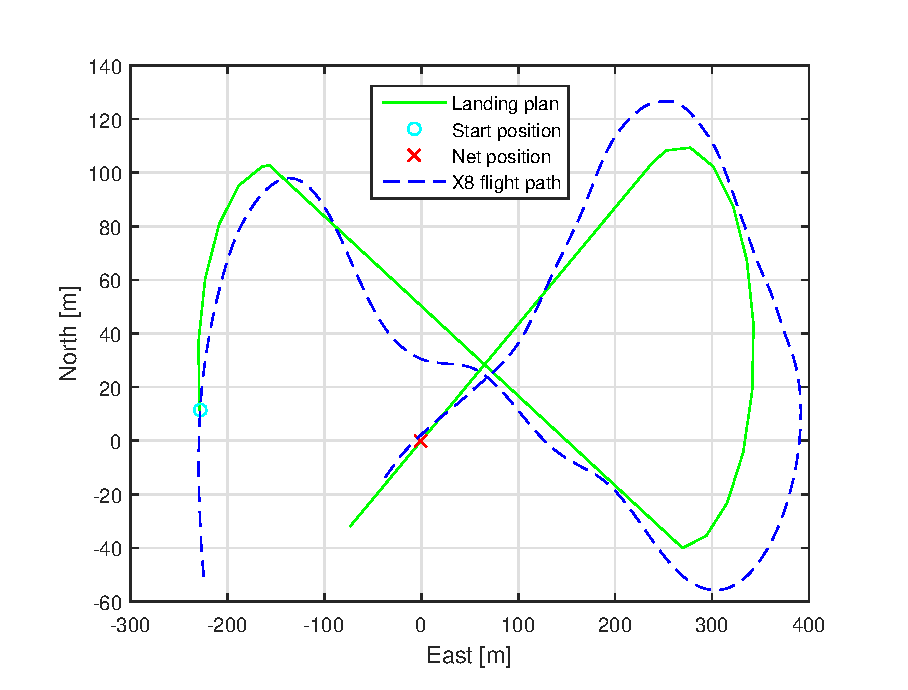
\includegraphics[scale=0.7]{figs/Experiment/NorthEast31mai103029.eps}
		\caption{North-East plot where the start and finish turning circles have opposite turning directions}
		\label{Fig:NorthEast31mai103029}
\end{figure}
\begin{figure}[H]
\centering
		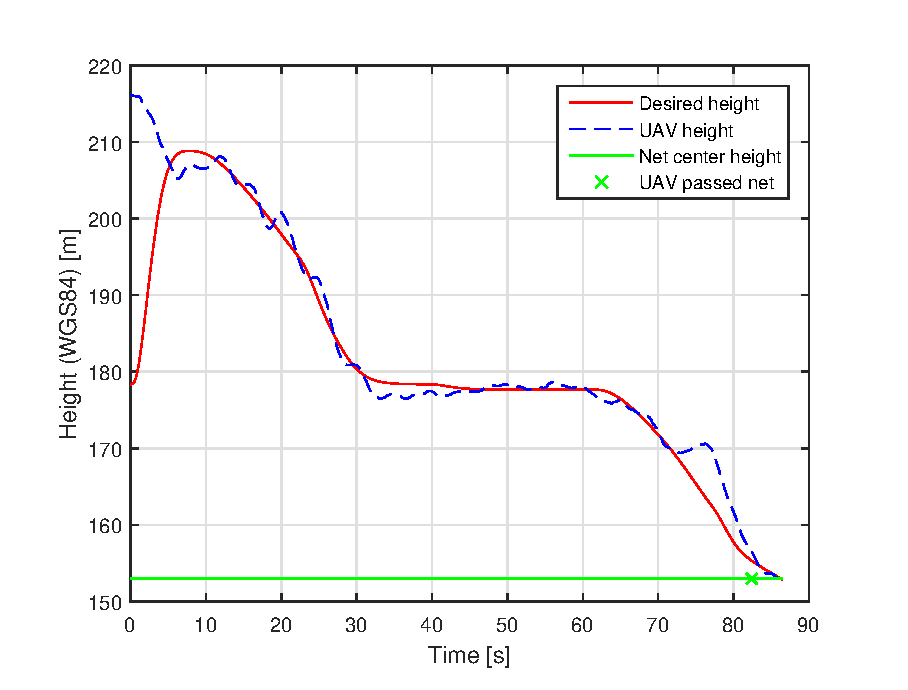
\includegraphics[scale=0.7]{figs/Experiment/Height31mai103029.eps}
		\caption{Height profile of a landing plan with $3 \deg$ net impact angle}
		\label{Fig:Height31mai103029}
\end{figure}
\subsubsection{Path with $\gamma_n = 0$}
A landing plan with the final approach angle ,$\gamma_n = 0$, was created, where the desired and actual height of the \gls{uav} is shown in figure\ref{Fig:Height31mai31mai105034}. The effect of setting the net impact angle to zero gave a better performance from the longitudinal control system, due to the desired height now converging to the net center height. At the time the \gls{uav} passed the virtual net the hight error with respect the height of the net center was within the height error acceptance.
\begin{figure}[H]
\centering
		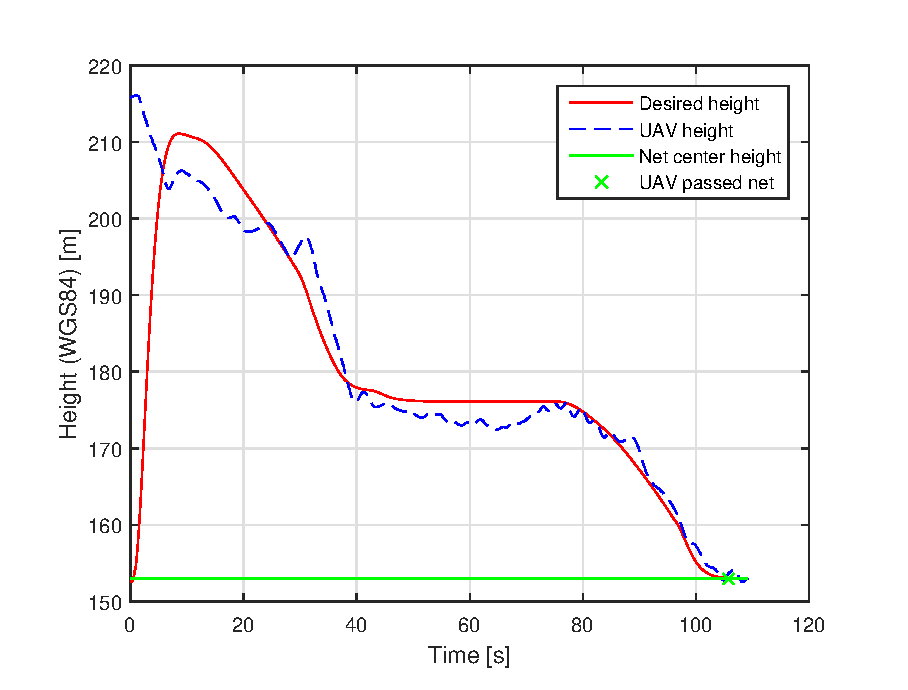
\includegraphics[scale=0.7]{figs/Experiment/Height31mai105034.eps}
		\caption{Height profile of a landing plan with $0 \deg$ net impact angle}
		\label{Fig:Height31mai31mai105034}
\end{figure}
\subsubsection{Path with inverted rotation direction in the start circle}
A landing plan with the rotation direction of the start turning circle inverted with respect to the previous landing plan, as shown in figure \ref{Fig:NorthEast31mai125420}. The result of this alteration was reduced oscillation in the lateral plane for the \gls{uav} when flying along the straight line between the turning circles. The \gls{uav} still experience overshot in the finish turning circle, however the overshooting is reduced due to more stable entry into the finish turning circle.
\begin{figure}[H]
	\centering
	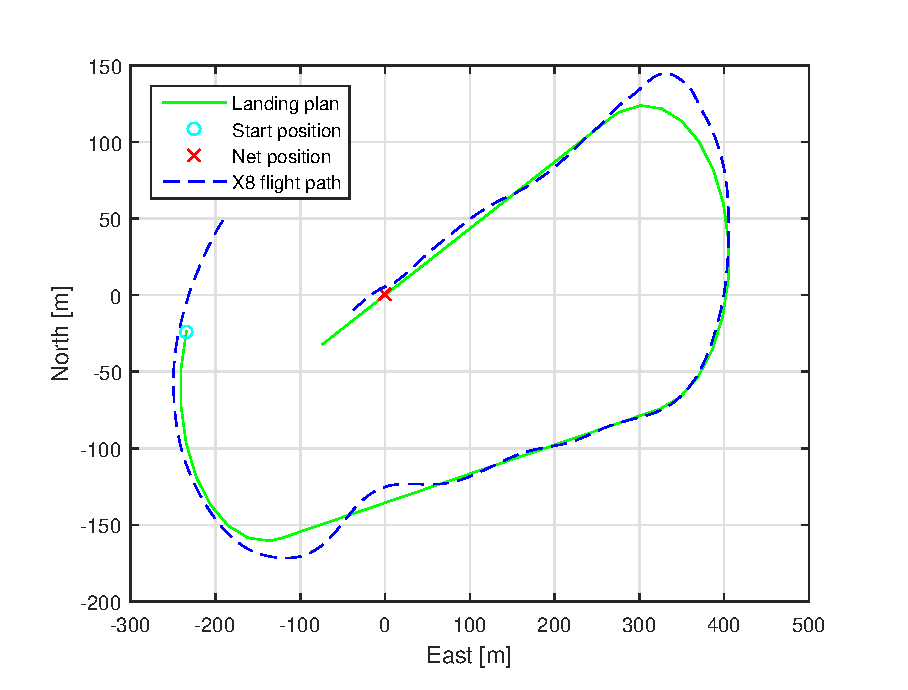
\includegraphics[scale=0.7]{figs/Experiment/NorthEast31mai125420.eps}
	\caption{North-East plot where the start and finish turning direction have the same turning direction}
	\label{Fig:NorthEast31mai125420}
\end{figure}
\subsubsection{Path with reduced lookahead distance in lateral controller}
In order to further reduce the oscillatory motion in the lateral plan the lookahead distance in the lateral control system was reduced to make the controller more aggressive towards the wind. The effect of this change is shown in figure \ref{Fig:NorthEast31mai131844}, where the oscillatory motion is almost completely removed. However the reduced lookahead distance did not affect the the overshot in the finish turning circle.
\begin{figure}[H]
\centering
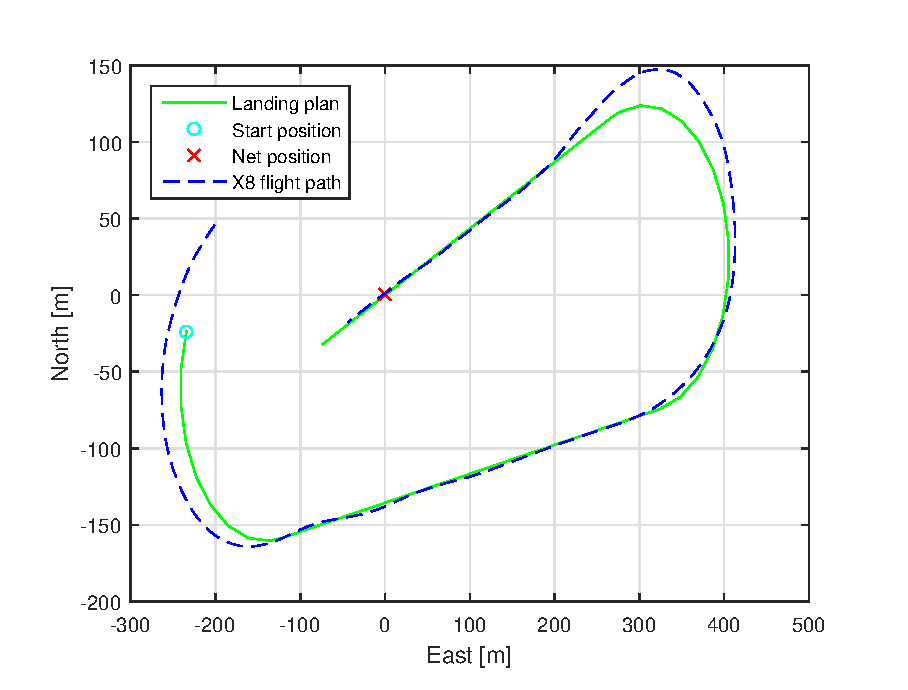
\includegraphics[scale=0.7]{figs/Experiment/NorthEast31mai131844.eps}
\caption{North-East plot where the lookahead distance of the lateral controller was reduced to increase performance of the autonomous landing system when flying against the wind}
\label{Fig:NorthEast31mai131844}
\end{figure}
By reviewing the desired roll ($\phi_d$ ) and the actual roll ($\phi$) of the \gls{uav} at the time of the final turn, shown in figure \ref{Fig:DesiredRoll131844}, it's observed that the lateral control system decrease the desired roll in the middle of the turn. This happens since the lateral control system only sees the next point on the circle, and not the circle as a whole.
\begin{figure}[H]
\centering
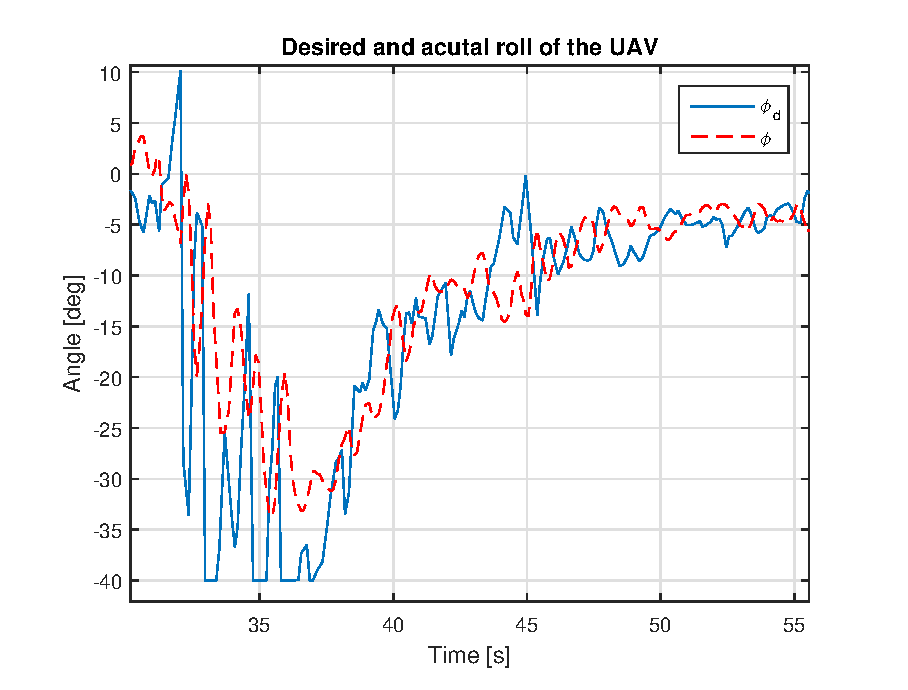
\includegraphics[scale=0.7]{figs/Experiment/rollDesired131844.eps}
\caption{The desired roll and actual roll of the \gls{uav} during the finish turning circle}
\label{Fig:DesiredRoll131844}
\end{figure}
\subsubsection{Summary of day 1}\label{sss:summaryDay1}
The result from the first day was affected with strong wind condition, in which the \gls{uav} struggled to stay on the path and overshooting in the finish turning circle. The heigh and cross track error for 11 landing plan missions, is given in table \ref{tb:Day1HeightCrossTrack}. The average height error vary less then the average cross track error, with a variance of $0.4 m$ against $6.2 m$. However the performance of the \gls{uav} in both height error and cross track error is worse then the results obtain during SIL simulation. This was expected, however the magnitude of the variance in the average cross track error shows that the performance of the lateral control system must increase in order for the autonomous landing system to be considered reliable. 
\begin{table}[H]
\centering
\begin{tabular}{| l | l | l |}
\hline
\textbf{Nr.} 	& \textbf{Average height error [m]} 	& \textbf{Average cross track error [m]}  \\ \hline
$1$				& $1.5$							& $6.1$								\\ \hline
$2$				& $2.6$							& $6.7$								\\ \hline
$3$				& $0.9$							& $5.5$								\\ \hline
$4$				& $0.1$							& $2.8$								\\ \hline
$5$				& $1.7$							& $2.0$								\\ \hline
$6$				& $1.3$							& $6.8$								\\ \hline
$7$				& $1,8$							& $9.1$								\\ \hline
$8$				& $1.2$							& $8.2$								\\ \hline
$9$				& $1.9$							& $5.9$								\\ \hline
$10$			& $1.5$							& $4.4$								\\ \hline
$11$			& $1.5$							& $1.4$								\\ \hline
Average			& $1.5$							& $5.4$								\\ \hline
Variance		& $0.4$							& $6.2$								\\ \hline
\end{tabular}
\caption{Mean height and cross track error from day 1}
\label{tb:Day1HeightCrossTrack}
\end{table}
The variance of the longitudinal control system shows that the control system is reliable in performance, however the average error must be reduced in order for the autonomous landing system to be able to hit the stationary net with increased probability of success. The results of whether the \gls{uav} was within the net acceptance criteria at the time of net passing, is given in table \ref{tb:Day1LandingAttempt}. Most of the alteration of the path and controller parameters was aimed towards the lateral control system, which is shown be be increased performance during the later attempts. In the comparison to the simulation results, where the average cross track error was almost zero, the performance has clearly decreased. This behaviour was expected due the simulation model used in the simulation has not been verified.
\begin{table}[H]
\centering
\begin{tabular}{| p{0.5cm} | p{1cm} | p{1cm} | p{3.5cm} | p{3cm} | p{1cm} |}
\hline
\textbf{Nr.}	& \textbf{Height error [m]}	& \textbf{Cross track error [m]}& \textbf{Height acceptance}& \textbf{Cross track error acceptance}	& \textbf{Net hit}\\ \hline
$1$				& $2.8$		& $2.1$		& X								& OK									& X					\\ \hline
$2$				& $2.7$		& $-4.5$	& X								& X										& X					\\ \hline
$3$				& $0.9$		& $-1.6$	& OK							& OK									& OK				\\ \hline
$4$				& $0.0$		& $5.4$		& OK							& X										& X					\\ \hline
$5$				& $0.8$		& $5.3$		& OK							& X										& X					\\ \hline
$6$				& $2.1$		& $-1.6$	& X								& OK									& X					\\ \hline
$7$				& $0.7$		& $2.3$		& OK							& OK									& OK				\\ \hline
$8$				& $-1.5$	& $-5.4$	& X								& X										& X					\\ \hline
$9$				& $1.9$		& $0.8$		& X								& OK									& X					\\ \hline
$10$			& $0.3$	& $1.1$		& OK							& OK									& OK				\\ \hline
$11$			& $-1.3$	& $0.2$		& OK							& OK									& OK				\\ \hline
\end{tabular}
\caption{Table containing the result of each landing attempt}
\label{tb:Day1LandingAttempt}
\end{table}
The content of table \ref{tb:Day1LandingAttempt} is shown in figure \ref{Fig:Day1NetPass}, where the net is marked as a whole line and all landing attempts are marked as crosses. The oscillatory motion in the lateral plane by the \gls{uav} is reflected in the placement of the crosses. However the placement of the cross shows the effect of an high average height error by either passing over the net or in the upper part of the net.
\begin{figure}[H]
\centering
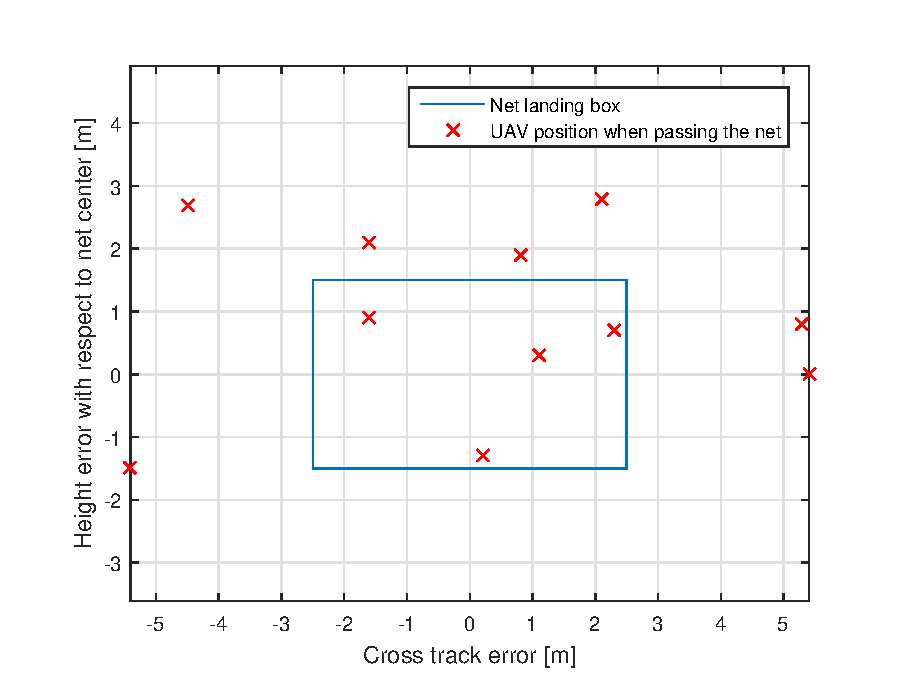
\includegraphics[scale=0.7]{figs/Experiment/day1NetHit.eps}
\caption{Position of UAV relative to the net center at the time of net passing}
\label{Fig:Day1NetPass}
\end{figure}
During the execution of the landing plan it was discovered that in order for the \gls{uav} to stay above the highest tree tops it had to start its decent from an height of $56 m$ above the airfield. Flying bellow this height would result in the pilot losing sight of the \gls{uav}, which is unacceptable in a LOS \gls{uav} operation. This didn't provide a problem during landing attempt with a virtual net which was placed $26 m$ above the airfield, however during a real stationary net landing it would push the limitation of the operation area in which the \gls{uav} can fly. A $56 m $ decent with a glide slope angle of $6\deg$ would require a glide slope of $500 m$. An estimate of the the available length of which the \gls{uav} can use to perform a autonomous landing in a stationary net is estimated to be $700 m$. This would require the use of the entire runway at Agdenes. An alternative solution is to attempt to land with a greater glide slope angle, or simply start the landing path from the west with respect to the runway. Landing attempts from the west has yet to tried, the reason being limited time and that would mean that the \gls{uav} would have to land in tail wind. This would increase the ground speed of the \gls{uav}, which is undesired. In the case where the wind is calm enough to be considered negligible, a autonomous landing from west would be a valid option.
\subsection{Day 2}
\subsubsection{First plan}\label{sss:Day2FirstPlan}
The second day had calm wind condition, which is considered as ideal field test conditions for the autonomous landing system. In an attempt to increase the height difference between the start height of the landing path and the net center, a longer glide slope was attempted. Among the alteration was moving the virtual net further to the west with respect to the runway, and the length and angle of the glide slope was increase to $280 m$ and $8 \deg$ respectfully. The full path specification for the first path is given in appendix \ref{AP:SpecDay2}. Figure \ref{Fig:NorthEast1juni081328} shows a North-East plot of the path created with the new specification, which show the lateral path overshoots both the start and finish turning circles. The overshot in the start circle is a result of the roll angle is not able to follow the desired roll angle fast enough, as seen in figure \ref{Fig:Roll1juni081328}, which is due to the low level roll controller being poorly tuned for autonomous flights where high precision performance from the \gls{uav} is desired. In addition the control surface used to control the roll of the \gls{uav} is also used to control the pitch, which results in having to weight the performance in heading against the ability to follow a height reference.
\begin{figure}[H]
\centering
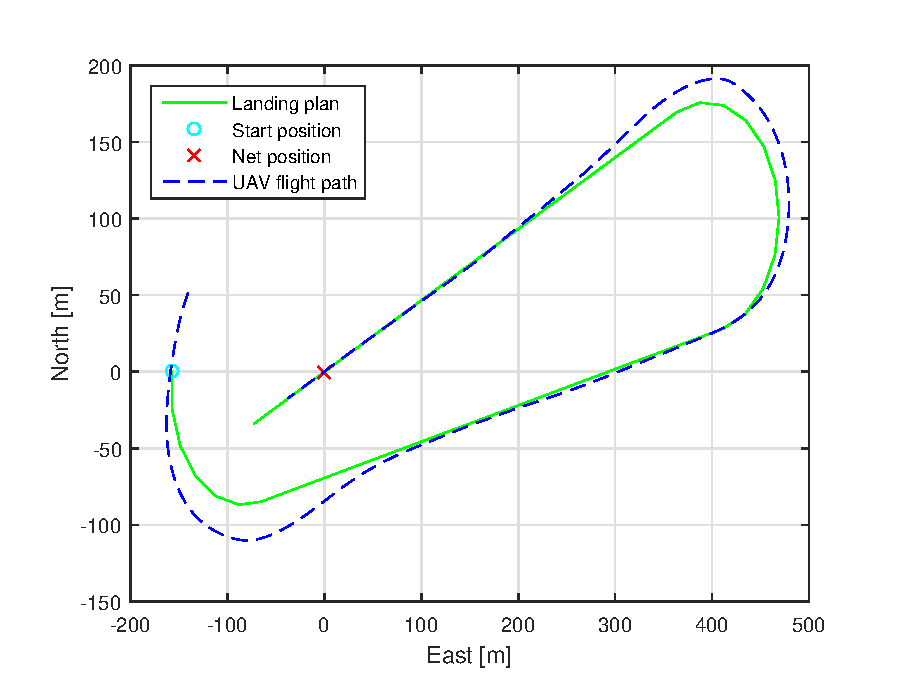
\includegraphics[scale=0.7]{figs/Experiment/NorthEast1juni081328.eps}
\caption{North-East plot created with the path parameter listed in table \ref{AP:SpecDay2}}
\label{Fig:NorthEast1juni081328}
\end{figure}
\begin{figure}[H]
\centering
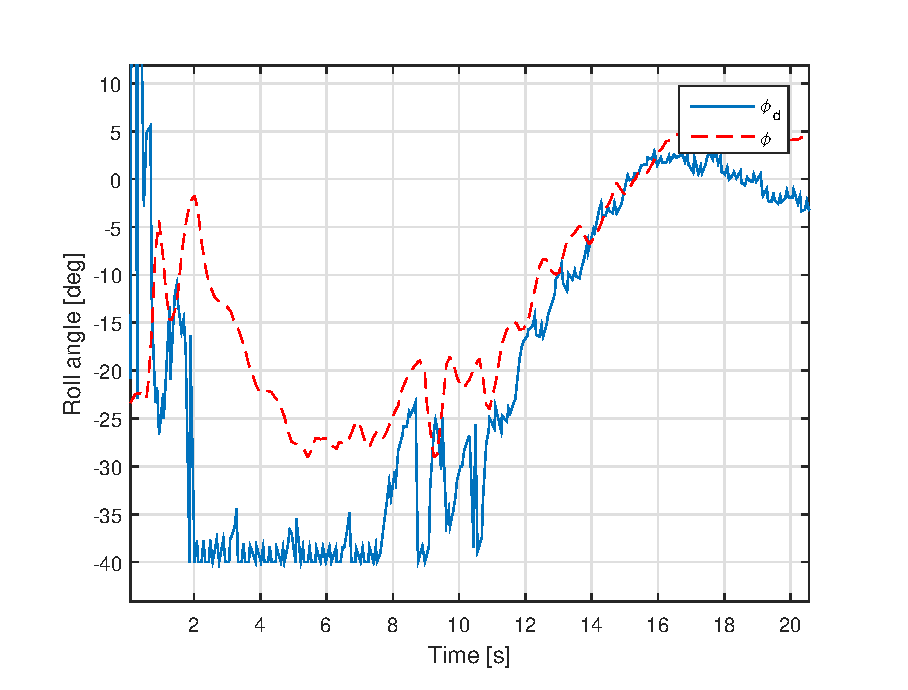
\includegraphics[scale=0.7]{figs/Experiment/Roll1juni081328.eps}
\caption{Desired and actual roll angle during the start turning circle}
\label{Fig:Roll1juni081328}
\end{figure}
The desired height and the actual heigh of the \gls{uav} is shown in figure \ref{Fig:Height1juni081328}, which shows that the \gls{uav} is unable to follow a glide slope with a slope angle of $\gamma_l = 8 \deg$. A key reason for this behaviour is due to the inability of the \gls{uav}s low level pitch controller to follow the desired pitch, as shown in figure \ref{Fig:Pitch1juni081328}. The pitch appear to be saturated in the low level controller since it does not attempt to reach the desired pitch. The low level pitch controller must be further fine tuned, and similar to the low level roll controller, has not been fine tuned for autonomous flights where high precision performance is desired.
\begin{figure}[H]
\centering
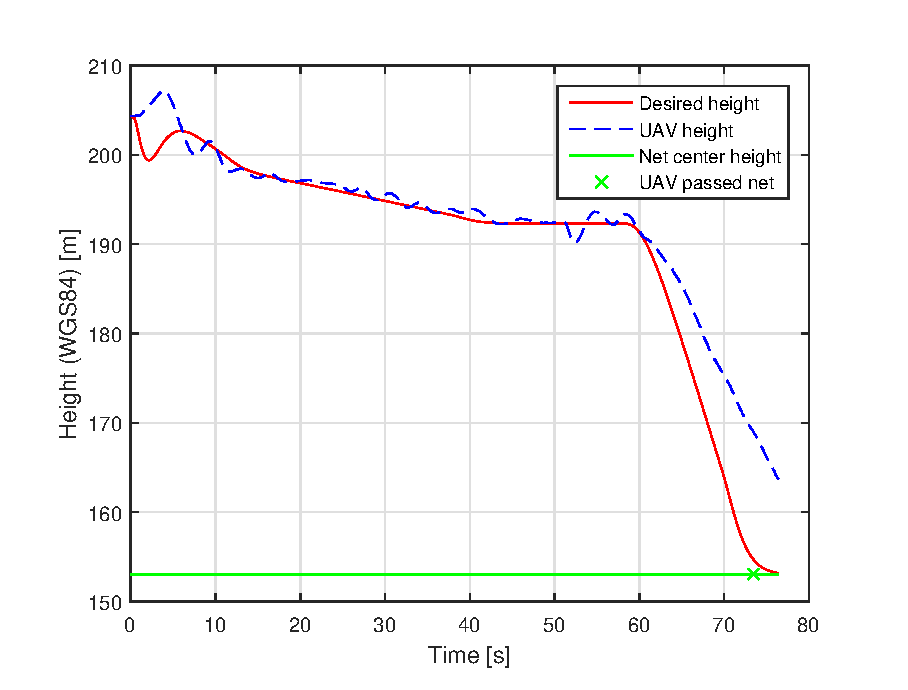
\includegraphics[scale=0.7]{figs/Experiment/Height1juni081328.eps}
\caption{Desired and actual height of the \gls{uav} with a glide slope angle of $\gamma_l = 8 \deg$}
\label{Fig:Height1juni081328}
\end{figure}
\begin{figure}[H]
\centering
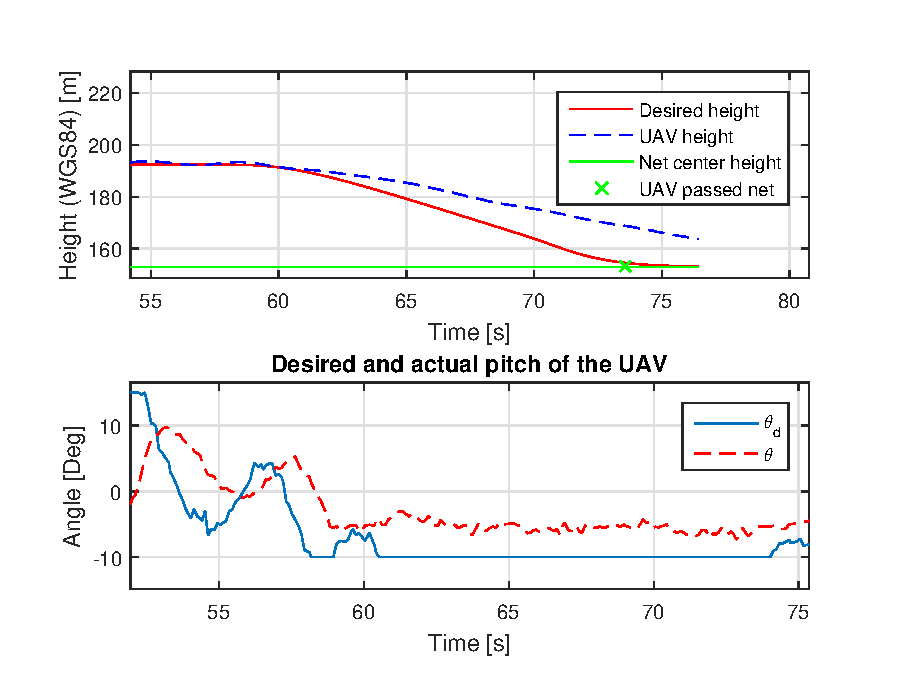
\includegraphics[scale=0.7]{figs/Experiment/Pitch1juni081328.eps}
\caption{Desired $\theta_d$ and actual pitch $\theta$, of the \gls{uav} at the time the \gls{uav} is in the glide slope}
\label{Fig:Pitch1juni081328}
\end{figure}
\subsubsection{Reducing arc segments distance}
In an attempt to further reduce the overshot in the finish turning circle the distance between each arc segments in the approach path circles was reduced from $25 m$ to $10 m$. The desired response with this alteration of the approach path was to ensure that the lateral control system keeps a high desired roll angle through the turning circle, thus reducing the overshot and increase the performance. A North-East plot of the resulting path is shown in figure \ref{Fig:NorthEast1juni083423}, which shows that the \gls{uav} has reduced its overshot in the final turning circle. The desired behaviour where the lateral control system keep a high desired roll angle through is achieved and shown in figure \ref{Fig:RollFinalTurning083423}. The confirmation that the \gls{uav} had a small overshot from the desired path is shown in the cross track error plot given in figure \ref{Fig:CrossTrackError1juni083423}.
\begin{figure}[H]
\centering
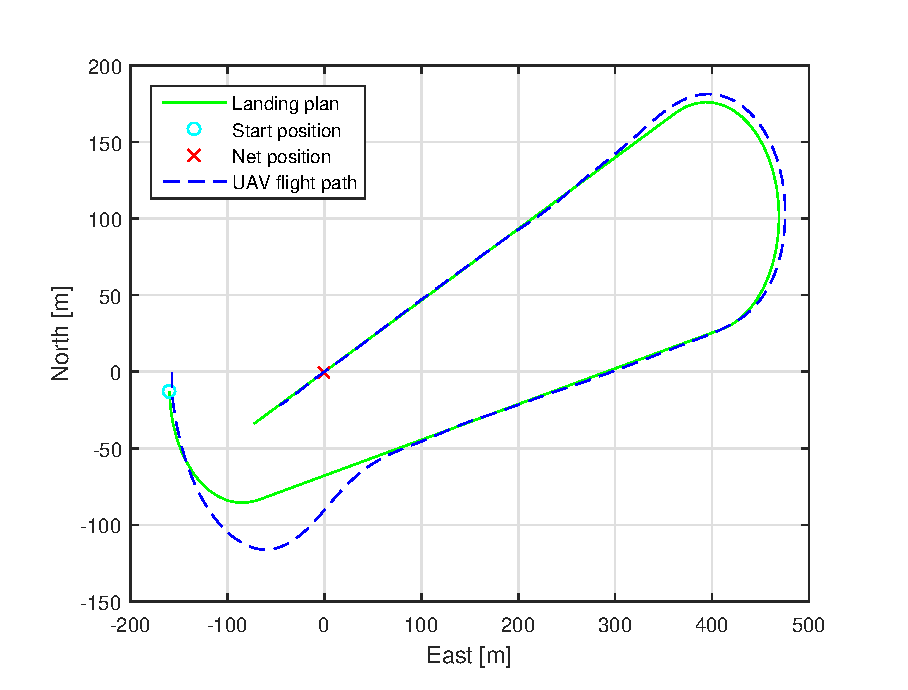
\includegraphics[scale=0.7]{figs/Experiment/NorthEast1juni083423.eps}
\caption{North-East plot where the distance between each arc segments has been reduced from $25 m$ to $10 m$}
\label{Fig:NorthEast1juni083423}
\end{figure}
\begin{figure}
\centering
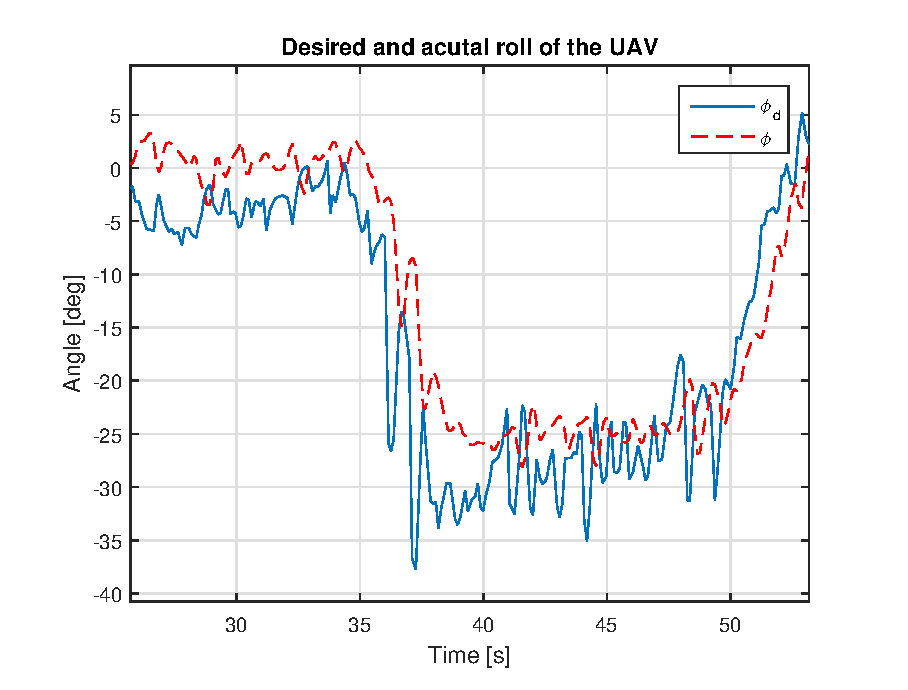
\includegraphics[scale=0.7]{figs/Experiment/Roll1juni083423.eps}
\caption{Roll and desired roll in the final turning circle}
\label{Fig:RollFinalTurning083423}
\end{figure}
\begin{figure}[H]
\centering
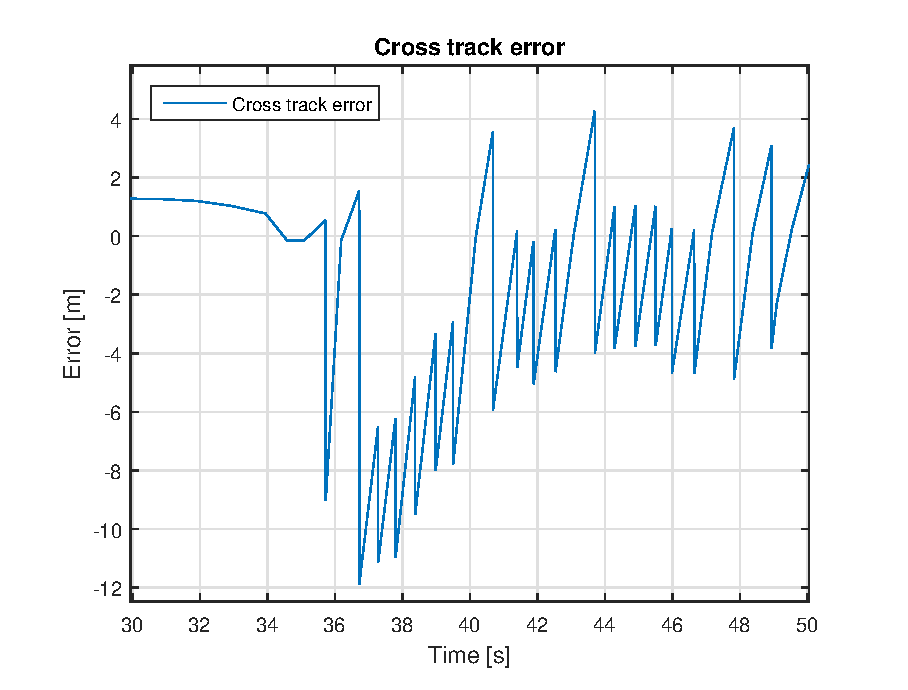
\includegraphics[scale=0.7]{figs/Experiment/CrossTrackError1juni083423.eps}
\caption{Cross track error in the final turning circle}
\label{Fig:CrossTrackError1juni083423}
\end{figure}
\subsubsection{Summary day 2}
The weather condition during the second day can be considered ideal for testing the autonomous landing system, thus possible to identify the strength and weaknesses of the system where the weather affect is negligible. The goal with the second day was to increase the height from which the \gls{uav} would start its decent towards the net by increasing the glide slope angle, and to investigate path parameter that can be used to reduce the \gls{uav}s overshot during turning in the final turning circle. The attempts to increase the glide slope angle during landing plan mission are reflected in table \ref{tb:Day2LandingAttempt}, which contain the results of whether the \gls{uav} passed through the net or not. Attempts with glide slope angles greater then $6 \deg$ resulted in the \gls{uav} to miss the net, however this performance could be increased with a better better tuning of the low level pitch controllers. With the current longitudinal control system the maximum glide slope angle which the X8 is able to follow during a autonomous landing is $6 \deg$. In addition increased performance from the longitudinal control system can be achieved by increasing the length of the final approach, in order for the \gls{uav} to have longer time to converge to the net center height. The final approach length could be increased to $120 m$ by moving the net to the edge of the runway at Agdenes. The risk with a large final approach during a autonomous landing in a real net would be the prolonged time the \gls{uav} flies $3-4 m$ above ground. A loss of high accurate positioning system could then result in a crash.

\begin{table}[H]
\centering
\begin{tabular}{| p{0.5cm} | p{1cm} | p{1cm} | p{3.5cm} | p{3cm} | p{1cm} |}
\hline
\textbf{Nr.}	& \textbf{Height error [m]}	& \textbf{Cross track error [m]}& \textbf{Height acceptance}& \textbf{Cross track error acceptance}	& \textbf{Net hit}\\ \hline
$1$				& $14.4$		& $0.1$		& X								& OK									& X					\\ \hline
$2$				& $1.3$		& $0.6$	& OK								& OK										& OK					\\ \hline
$3$				& $1.1$		& $-0.2$	& OK							& OK									& OK				\\ \hline
$4$				& $1.4$		& $0.1$		& OK							& OK										& OK					\\ \hline
$5$				& $1.1$		& $0.1$		& OK							& OK										& OK					\\ \hline
$6$				& $2.0$		& $-0.2$	& X								& OK									& X					\\ \hline
$7$				& $2.3$		& $0.2$		& X								& OK									& X				\\ \hline
$8$				& $7.0$	& $0.3$	& X										& OK										& X					\\ \hline
\end{tabular}
\caption{Table containing the result of each landing attempt}
\label{tb:Day2LandingAttempt}
\end{table}
The lateral control system perform better compared to the first day during calm wind condition which is reflected in the table \ref{Tb:AverageCrossHeightDay2}, where the performance from 8 landing plan missions is presented. The performance from the longitudinal control system remain similar to the first day, which shows that the longitudinal control system is less affected by the wind then the lateral control system, however the the average height error of the longitudinal control system must be decreased in order for the autonomous landing to achieve a higher probability of successfully performing a successful net landing. The high average height error of the longitudinal control system is reflected in figure \ref{Fig:Day2NetPass}, where those crosses that are within the height acceptance criteria are in the upper part of the net.
\begin{table}[H]
\centering
\begin{tabular}{| l | l | l |}
\hline
\textbf{Nr.} 	& \textbf{Average height error [m]} 	& \textbf{Average cross track error [m]}  \\ \hline
$1$				& $2.2$							& $3.8$										\\ \hline
$2$				& $1.2$							& $3.4$										\\ \hline
$3$				& $0.9$							& $-1.8$									\\ \hline
$4$				& $2.5$							& $-0.2$									\\ \hline
$5$				& $3.0$							& $0.3$										\\ \hline
$6$				& $1.6$							& $0.2$										\\ \hline
$7$				& $1,9$							& $-2.3$									\\ \hline
$8$				& $1.9$							& $-0.1$									\\ \hline
Average			& $1.9$							& $0.5$										\\ \hline
Variance		& $0.5$							& $4.7$										\\ \hline
\end{tabular}
\caption{Average height and cross track error from day 2}
\label{Tb:AverageCrossHeightDay2}
\end{table}
\begin{figure}[H]
\centering
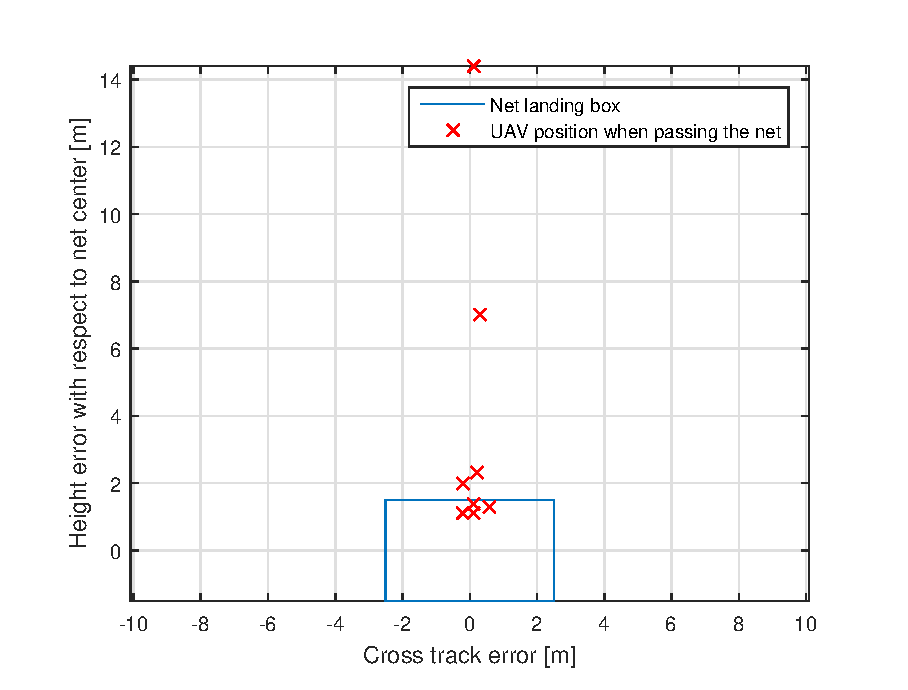
\includegraphics[scale=0.7]{figs/Experiment/day2NetHit.eps}
\caption{Position of the \gls{uav} relative to the net center at the time of net passing}
\label{Fig:Day2NetPass}
\end{figure}
\section{Navigation}\label{ss:NavigationResults}
\subsection{RTK-GNSS performance}
The performance from the \gls{rtk-gnss} system during both day of testing the autonomous landing system resulted in similar performance, thus only results from the first day is presented in this section, while the results from the second day is given in appendix \ref{AP:ADDResults}. The results from the \gls{rtk-gnss} system during the landing plan flights is summarised in table \ref{TB:RTKFirstDayRTK}, where the result is presented as percentage of the total number of GpsFixRtk messages.
\begin{table}[H]
\centering
\begin{tabular}{| l | l | l | l |}
\hline
\textbf{Nr.}	& \textbf{FIX \%}	& \textbf{FLOAT \%}	& \textbf{NONE \%}	\\ \hline
$1$				& $99.5 $	& $0.5$	& $0.0$									\\ \hline
$2$				& $99.5 $	& $0.5$	& $0.0$									\\ \hline
$3$				& $99.8 $	& $0.0$	& $0.0$									\\ \hline
$4$				& $100$		& $0.0$	& $0.0$									\\ \hline
$5$				& $100$		& $0.0$	& $0.0$									\\ \hline
$6$				& $100$		& $0.0$	& $0.0$									\\ \hline
$7$				& $99.9$	& $0.1$	& $0.0$									\\ \hline
$8$				& $99.7 $ 	& $0.3$	& $0.0$									\\ \hline
$9$				& $99.3$	& $0.7$	& $0.0$									\\ \hline
$10$			& $100$		& $0.0$	& $0.0$									\\ \hline
$11$			& $100$		& $0.0$	& $0.0$									\\ \hline
\end{tabular}
\caption{Performance of the RKT-GNSS system the first day during the executing of the landing plans}
\label{TB:RTKFirstDayRTK}
\end{table}
\subsection{Short loss compensator}
The short loss compensator was engaged during a flight where the \gls{rtk-gnss} started to experience problem. The flight plan was part of cooperative net recovery system presented in \citep{Sigurd} and \citep{Jostein}, which experience reduced \gls{rtk-gnss} performance due to decreased satellite geometry. During the flight the \gls{rtk-gnss} system experienced a drop out, as seen in figure \ref{Fig:NavSource}. The main reason for the drop out is shown in figure \ref{Fig:SatCount1juni114124}, where at the time of \gls{rtk-gnss} drop out the number of valid satellites starts to vary rapidly. Even though the \gls{rtk-gps} position solution is unavailable the navigation system is still able to supply high accurate position solution due to the short \gls{rtk-gnss} compensator as seen in figure \ref{Fig:ShortLoss}.
\begin{figure}[H]
\centering
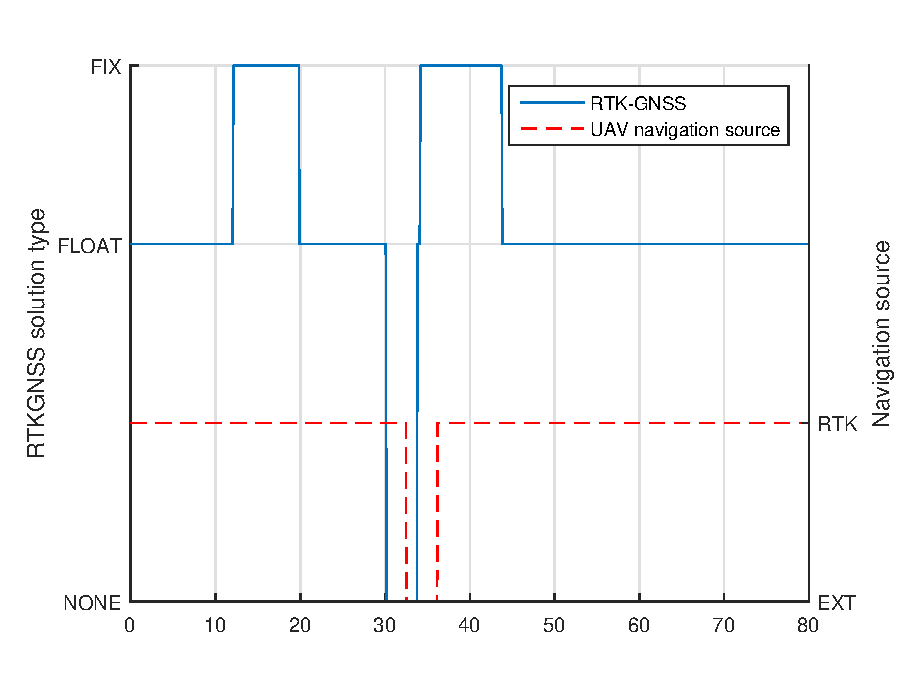
\includegraphics[scale=0.7]{figs/Experiment/navSource.eps}
\caption{State of RTK-GNSS system and \gls{uav} navigation source.}
\label{Fig:NavSource}
\end{figure}
\begin{figure}[H]
\centering
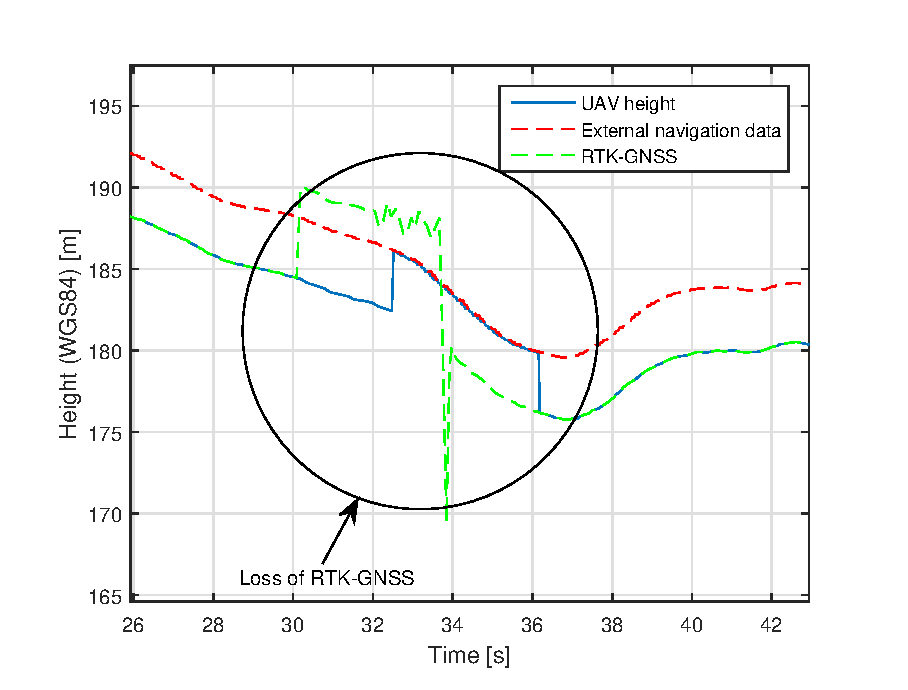
\includegraphics[scale=0.7]{figs/Experiment/shortrtkloss1juni114124.eps}
\caption{Loss of \gls{rtk-gps} triggers the short loss compensator such that the \gls{uav} keeps the \gls{rtk-gps} position solution longer}
\label{Fig:ShortLoss}
\end{figure}
\begin{figure}
\centering
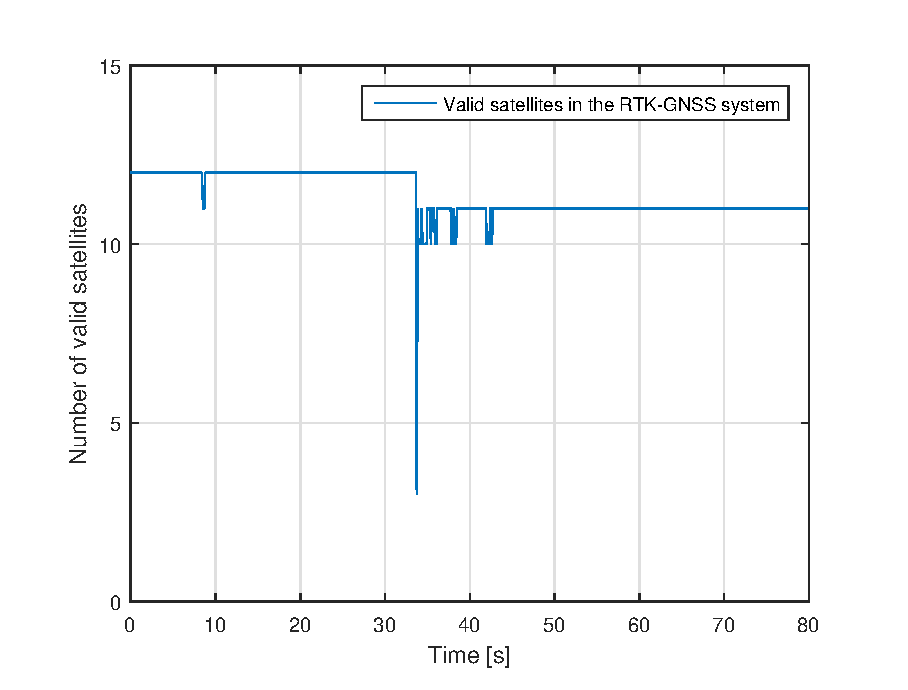
\includegraphics[scale=0.7]{figs/Experiment/ShortrtklossSatellites1juni114124.eps}
\caption{Number of valid satellites during a flight mission}
\label{Fig:SatCount1juni114124}
\end{figure}
\subsection{Summary of navigation system performance}
The navigation system was able to provide high accuracy position solution to the \gls{uav} during the autonomous landing flight plan, however continues drop out of the \gls{rtk-gnss} system was experienced when the satellite geometry decreased, which make the positioning system more susceptible to atmospheric disturbance. The continues drop out could be reduced by increasing the elevation mask in RTKlib, however this would limit the valid satellites to a number where a FIX solution from the \gls{rtk-gnss} system is no longer available. In order for the system to be able to perform during a prolong duration of degraded satellite geometry a state estimator must be created which can give a accurate position estimate with minimum \gls{rtk-gnss} information available. This would be a more advance estimator compared to the short loss compensator presented in this thesis.

The short loss compensator was able to compensate the solution from the external navigation system sufficiently to avoid a large step in \gls{uav} position data for the short period where the \gls{rtk-gnss} data was not available. However the limits of the short loss compensator has yet to determined, and should be further tested. The goal of the navigation system is be to be able to provide high accurate position solution to the \gls{uav}, even if the \gls{rtk-gnss} system experience a drop out.
\section{Summary}
This chapter has presented the result from the experimental testing of the autonomous landing system for a X8 fixed-wing \gls{uav} over the course of two days with different weather, where the landing target was a virtual net placed $26 m$ above the runway. The different weather condition allowed for identification of strength and weaknesses with the control system, in addition to how alteration of landing plan parameters could affect the performance of the control system.

The longitudinal control system showed a stable performance, however a large average error in the height with respect to the desired height shows a performance that is not acceptable for a autonomous landing system. Compared to the results obtain in the SIL simulation \ref{SIL:Results} where the low level controllers are fined tuned, shows that the performance can be increased by further tuning of the low level pitch controller. This might allow for an increased glide slope angle, which will increase the height difference between the landing net and the start of the landing path or reduce the necessary glide slope length. However the risk with an increased glide slope angle is an increased airspeed, which could result in a large overshot with respect to the desired height. 

The lateral control system performed with satisfying result during the second day when the wind condition was calm, however during the first day it experienced problems when attempting to converge to the straight line between two waypoints. This result differ from the SIL simulation of the autonomous landing system, which was expected due to the mathematical model used to represent the X8 \gls{uav} has not been verified against a physical model of the X8, in addition to the low level controllers not being fined tuned for autonomous flights. The lateral control system  struggeled to avoid overshooting when following the finish turning circle, with some resulting overshot large enough to bring the \gls{uav} to the edged of the operational flight space. During the flight experiments some key factors was identified which resulted in increased performance from the lateral control system. The key factors are listed in table \ref{Tb:KeyAlterationFactorsLateral}.
\begin{table}[H]
\begin{itemize}
\item Reducing the lookahead distance when flying in strong wind conditions.
\item Creation of a approach path with the same rotation direction in both turning circles.
\item Reducing the distance between each arc segments in the turning circles.
\end{itemize}
\caption{Alteration in the autonomous landing system which resulted in increased performance from the lateral controller}
\label{Tb:KeyAlterationFactorsLateral}
\end{table}
The reduction of the lookahead distance will result in increased performance when against the wind, at the cost of reduced performance when flying in the tail wind. A possible solution to this problem would be to implement the the lookahead distance as a function of the cross track error, which in \citep{fossen2011handbook} section 10.3.2 is given as:
\begin{equation}
\Delta(t) = \sqrt{R^2 - e(t)^2}
\end{equation}
where $\Delta(t)$ is the lookahead distance, $R$ is the maximum lookahead distance and $e(t)$ is the cross track error. In addition the lateral control system functionality could be expanded to increase the performance during a turning manoeuvre, with the goal of reducing the overshot.

Experimentation with the landing plan parameter showed that both the lateral and longitudinal control system was affected by the choice of parameters. During the first day the rotation direction of the start turning circle brought the \gls{uav} into the cross wind, which caused oscillatory motion in the \gls{uav}. Thus the combination of rotation direction should be considered carefully, with the recommended combination being either counter-clockwise/counter-clockwise or clockwise/clockwise. These combinations will result a smoother transition between the two turning circles, hence reduce the oscillation in the lateral controller. In addition the final approach angle must be zero, in order for the longitudinal control system to output a desire height reference which equals the net center height. Other key landing plan factors with recommended values for increase autonomous landing system performance are listed in table \ref{Tb:RecommmendedLandingPlanParameter}.
\begin{table}[H]
\centering
\begin{tabular}{| l | l |}
\hline
\textbf{Parameter name}			&  \textbf{Recommended value} 	\\ \hline
Time of arrival factor			&	$2 s$						\\ \hline
Distance between arc segments	&	$10 m$					 	\\ \hline
Final approach length			&	$100 m$					 	\\ \hline
Final approach angle			&   $0 \deg$					\\ \hline
Glide slope angle				&	$6 \deg$				 	\\ \hline
\end{tabular}
\caption{Recommended parameter alteration to the landing plan with respect to the plan parameter given in table \ref{AP:TB:landingDay2}, and the task configuration parameter given in table \ref{Tb:LandingPlanParameter}}
\label{Tb:RecommmendedLandingPlanParameter}
\end{table}
The minimum height from which the autonomous landing system could start the landing path from was found to be $56 m$ above the runway at Agdenes airfield when attempting to land from the east. This strain the operation boundaries in which the \gls{uav} operates, since the approach could move the \gls{uav} out of the line of sight of the pilot. An alternative approach from the west is possible, however the typical wind condition on Agdenes is from the west, which would limit the weather window of the autonomous landing system.

The navigation system performed with satisfying results, and showed that it's able to provide a stable and reliable \gls{rtk-gnss} solution to the navigation system. However the \gls{rtk-gnss} is still prone to bad satellite geometry, which will result in the \gls{rtk-gnss} system to loose lock of the satellites. During these events the short \gls{rtk-gnss} loss compensator is able to compensate the external navigation system, such that the navigation position solution remain at the same accuracy level as with \gls{rtk-gnss}. The time limitation in which the compensator is able to operate without divergence from the \gls{rtk-gnss} accuracy level has yet to determined.